\chapter{IoT}
L'Internet delle cose (Internet of Things, IoT) è un paradigma riferito
all’estensione di internet al mondo degli oggetti. Nel 1999 il ricercatore
britannico Kevin Ashton, durante una presentazione, teorizzò  per primo un mondo
nel quale oggetti ,dotati di sensori, interagiscono utilizzando la rete.  La
continua evoluzione delle tecnologie wireless e satellitari ha permesso
l'ideazione di oggetti sempre più connessi, in grado di generare una grande mole
di informazioni e dati. Oltre ai computer,smartphone e tablet, sempre più
oggetti di uso quotidiano dispongono di una connessione ad internet. Smartwatch
e smart band , lampadine e prese elettriche "intelligenti" ,  sono già da tempo
reperibili nel mercato\bx{,} con un prezzo accessibile alla stragrande maggioranza dei
consumatori.  Data la bassa
complessità del hardware ,implementato in questi devices, necessitano di
appoggiarsi ad un server esterno per l'elaborazione dei dati.  Sfruttando la
connessione ad internet, gli oggetti riescono ad instaurare uno scambio di dati
bidirezionale tra loro ed il server. Il dispositivo, infatti,  dopo aver
convertito la grandezza fisica di suo interesse in un dato comprensibile al
server, invia l'informazione \bx{a quest'ultimo}, il quale, dopo un'elaborazione della
stessa, formulerà dei comandi di risposta all'oggetto.
\\
\begin{figure}[h]
        \centering 
                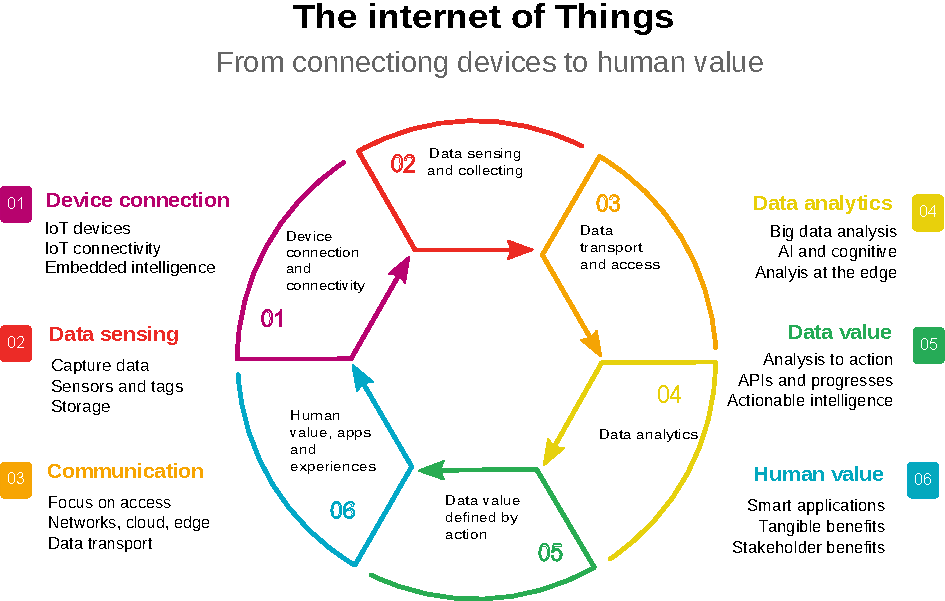
\includegraphics[width=16cm]{IoT-c1}
        \caption{Catena del valore dell'IoT}
        \label{fig:IoT_chain}
\end{figure}
I dati sono la materia prima del mondo dell'IoT, sono \bx{loro} che giocano il ruolo
principale sulla catena del valore (value chain), figura \ref{fig:IoT_chain},
dando una svolta importante ,dal
punto di vista economico, a nuovi settori quali il \emph{data mining} e la
\emph{business analysis}.
Attraverso lo studio delle informazioni presenti ,si potrà  aumentare l’efficienza di un
servizio oppure  migliorare la esperienza d'uso di una applicazione.
Muovendoci verso un modo sempre più connesso, nove problematiche riguardanti la
privacy e la sicurezza emergo.  Molto spesso, per tagliare i costi di produzione e
di sviluppo di questi gadget tecnologici, le aziende tendo a ridurre gli
investimenti nell'R\&D (Ricerca e Sviluppo), andando a produrre dispositivi con
un software non aggiornato o con componenti hardware di bassa qualità. Inoltre
, il ciclo vitale di un prodotto, non sarà più determinato solo dalla
rottura o dal mal funzionamento del dispositivo stesso ma, verrà ridotto dalla
impossibilità di un aggiornamento del firmware.
Le falle di sicurezza presenti nel software , ed il sempre più alto numero di
attacchi hacker, rappresentano un grave  pericolo per la sicurezza e la privacy del utente
finale.
È necessario quindi trovare un accordo, tra case produttrici e
consumatori ,al fine di garantire una \bx{life span minima}, di alcuni anni, per quanto
riguarda gli aggiornamenti. Riducendo così quello che più comunemente
viene chiamato il fenomeno della obsolescenza programmata. 
\section{Big Data}
Oltre all'innumerevole quantità di dati che verrà prodotta da questi milioni di
devices intelligenti, noi stessi,  navigando il web, ne produciamo una grande
quantità. Nel 2013\bx{,} si è stimato che ogni secondo nel web venivano generati una
quantità di dati pari a 28875GB . Con il  termine Big Data, si vuole
rappresentare l'insieme di tutti i dati eterogenei\bx{,} che ogni giorno vengono
prodotti e scambiati nella rete.
Con il progredire della tecnologia il dataset (aggregazione di dati) a
disposizione delle aziende è in continuo aumento.
Secondo un articolo pubblicato da Verizon, si stima che il 92\% delle aziende
usa meno del 25\% dei dati raccolti e che solo la metà  di esse prevede di
riuscire a fare fruttare una percentuale maggiore di quella attuale,nei prossimi due anni
\cite{Verizon}.  Con “Data mining” o "Data analytics"  si identificano tutte le
tecniche e le metodologie finalizzate all’estrazione di sapere e conoscenza
partendo da una vasta mole di dati.
L’enorme disponibilità, di ogni sorta di informazione, è una prospettiva che 
apre innumerevoli scenari di ricerca; ad esempio, predire con largo anticipo i 
trend del mercato, permetterebbe ,ad una azienda, di investire in maniera più
efficace le proprie risorse, andando a creare un maggiore profitto.


\section{La diffusione dell'Internet delle cose}
Nel 2008\bx{,} il numero di oggetti quali personal-computer, server, telefoni cellulari,
connessi ad internet, ha superato il numero di persone presenti nell'intero
pianeta. Il continuo sviluppo tecnologico, la sempre maggior facilità d'uso e
l'abbattimento dei costi, ha reso disponibile, al mondo consumer, tecnologie che
fino a poco tempo fa erano destinate ad un uso aziendale ed universitario. 
Con l'avvento dell'IoT, si prevede una crescita esponenziale di devices connessi
ad Internet;  secondo  una stima da parte di Gartner, il numero di smart
device presenti nell'anno 2020, sarà superiore a 20 miliardi \cite{gartner2016}.
Per fronteggiare una crescita così esponenziale, è d'obbligo cercare soluzioni
in grado di prevenire il congestionamento della rete. 
\\
\begin{table}[h]
        \centering
        \begin{tabular}{l|c|c|c|c}
                \textbf{Categoria}  & 2016 & 2017 & 2018 & 2019 \\
                \hline
                \emph{Consumer}  & 3963 & 5244,3 & 7063,3 & 12863 \\
                \emph{Business}  & 1418 & 2135.4 & 4152,7 & 6171  \\
                \emph{Totale }   & 6381 & 8380   & 11196  & 20415 \\
        \end{tabular}
        \caption{Stima di dispositivi IoT (Milioni di unità)
        Gartner\cite{gartner2016}}
\end{table}
\\
\begin{figure}[h]
        \centering 
                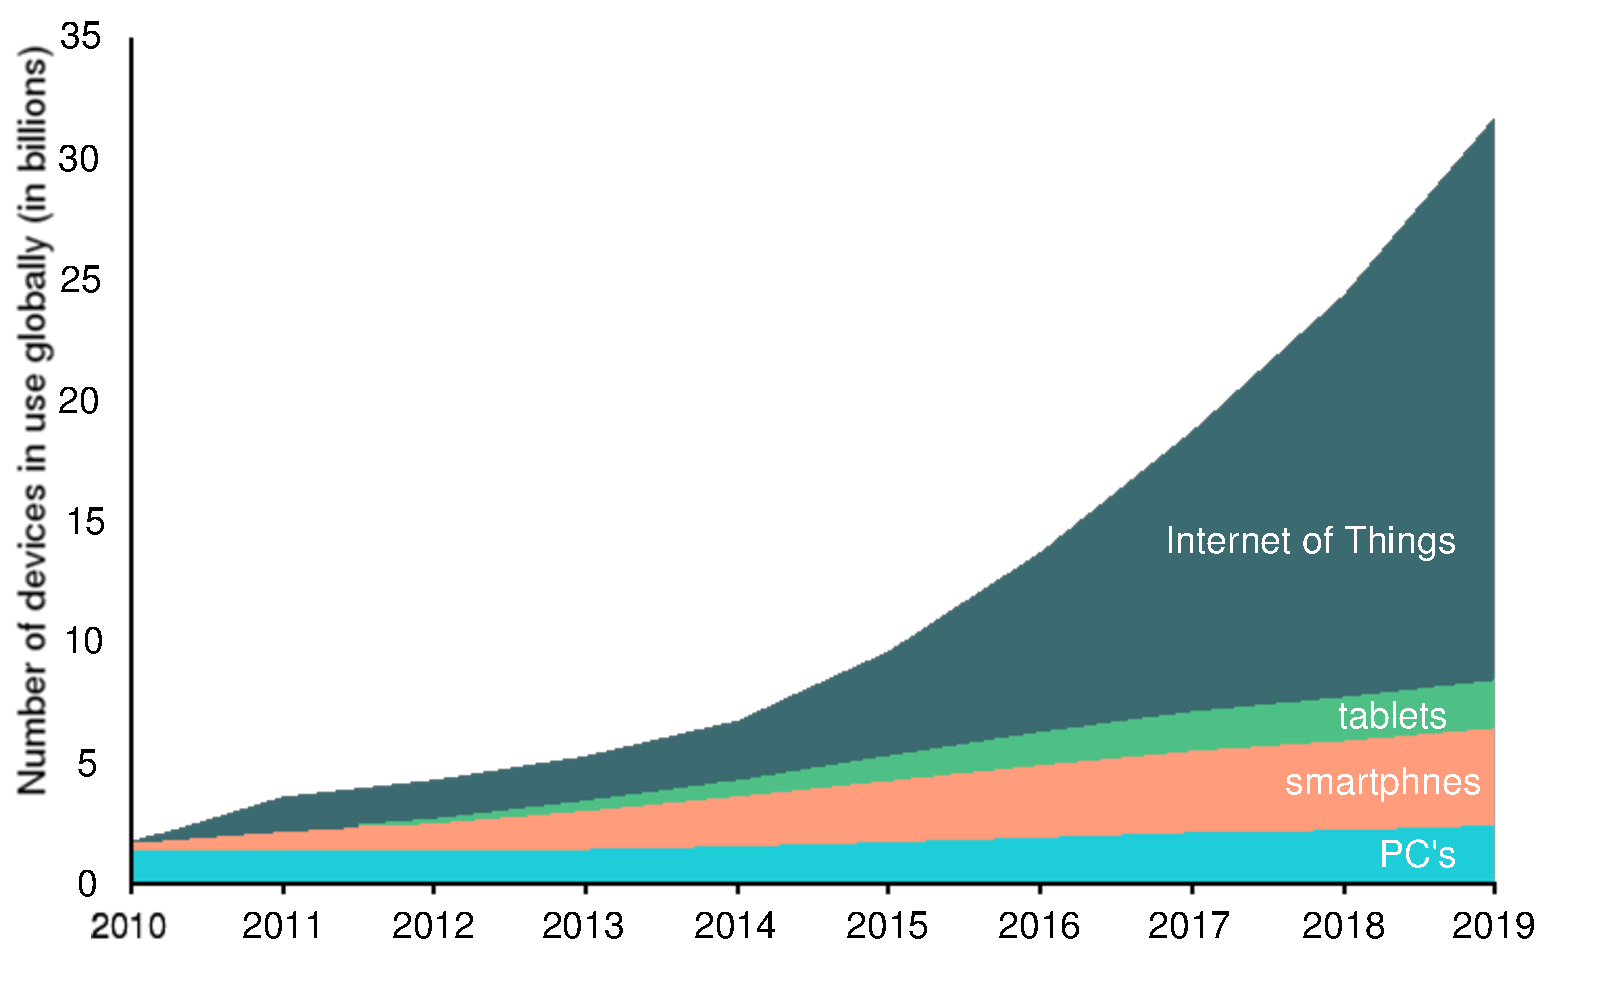
\includegraphics[width=10cm]{iot_devices}
        \caption{Numero di dispositivi per anno}
\end{figure}

\section{Business}
Considerando le statistiche precedenti, è comprensibile che l'IoT sia un
mercato che agisce in maniera trasversale su tutti i settori.  Se l'utilizzo di
sensori in ambiti quali la domotica e l'automotive è da tempo largamente
impiegato, grazie all'abbattimento del costi del
singolo  dispositivo e la facile implementazione di queste nuove tecnologie,  nuovi
mercati e nuove possibilità di investimento sono nate. Prendiamo come esempio
l'agricoltura di precisione, che grazie a sensori in grado di rilevare dati
riguardanti l'umidità del suolo, l'indice di piovosità oppure l'umidità fogliare,
permette all'agricoltore di  capire quando è il momento di intervenire per il
trattamento delle colture. In questo modo è possibile dispiegare le risorse in
maniera più efficace, andando ad agire solo nelle culture danneggiate.Sempre
secondo quanto stimato da Gartner, ci si aspetta che entro il 2020, 
la cifra investita nell'idustria del IoT,
sarà pari a circa \$3,000,000 milioni di dollari con un investimento annuo di
circa \$500,000 milioni di dollari. È utile osservare, che la più grande fetta e quella
riservata al mercato consumer dove smart TV, set-top box e smart cars saranno i prodotti
maggiormente richiesti.
\cite{gartner2016}. 



\section{La tecnologia alla base dell'IoT} 
Nell'industria il concetto di M2M (Machine to Machine) non è un concetto nuovo,
già Kevin Ashton, durante la presentazione in cui introdusse il termine IoT,
comprese le potenzialità della tecnologia RFID applicate alla supply chain. Dal
1999 ad oggi molte cose sono cambiate, ma molte domande non hanno ancora trovato
una risposta. Come accadde agli albori di Internet, quello che manca al modo
dell'IoT è una standardizzazione dei protocolli e del linguaggio con cui questi
oggetti devono comunicare. Astraendoci dal problema e portandoci ad una visione
di più alto livello problema, è possibile individuare in questo paradigma
tre livelli.
\begin{figure}[h]
        \centering 
                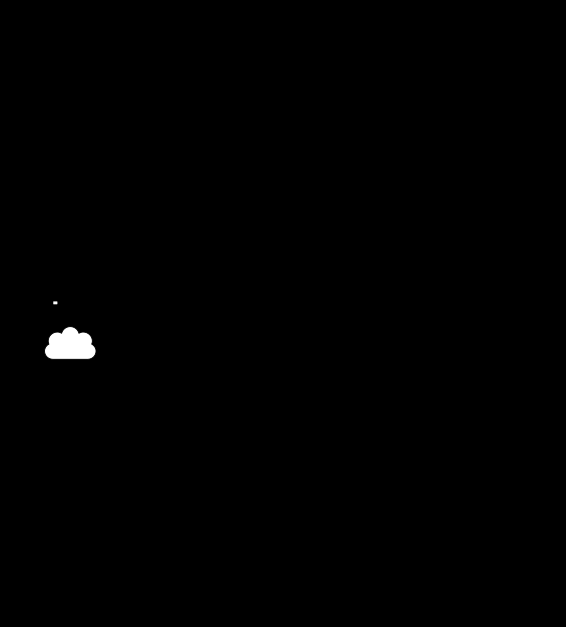
\includegraphics[width=10cm]{three-layer}
        \caption{Layer del IoT}
\end{figure}
\begin{itemize}
\item \textbf{Device layer} o sensor layer, è il layer più basso. Esso raggruppa
tutti i gli oggetti "smart". Questo layer è quello che mette in comunicazione il
mondo reale con gli atri layer superiori. A loro spetta lo scopo di convertire
una misura fisica in un segnale interpretabile da altri calcolatori.
La maggior parte di questi sensori, utilizzerà una connessione Bluetooth,
ZigBee, Wifi o una si baserà su una rete LPWAN per comunicare il dato al layer
superiore.
\item \textbf{Network layer} o mediation layer raggruppa l'intera infrastruttura
di rete e gateway che ricevono i dati da i vari sensori. Questo layer è
semplicemente un layer di mediazione dove l'informazione (dato) non viene altera
ma semplicemente trasmesso all'Application layer.
\item \textbf{Application layer} è il layer nel quale l'informazione viene
immagazzinata ed elaborata. Questo layer è il più importante, e qui dove il dato
viene trasformato da una semplice misurazione fisica ad una possibile revenue
per l'azienda che lo gestisce.%\improvement{Riscrivere}
\end{itemize}
Già molte sono le aziende che si sono mosse per cercare di imporsi in questo
mercato fiorente. Data la vastità dei campi di applicazione, non è semplice
prevedere quale standard predominerà sugli altri.
Aziende del calibro di Samsung con la
piattaforma \href{https://www.artik.io}{artik}  , Zigbee con
\href{https://www.speakdotdot.com/dotdot/}{DotDot} e Google con
\href{https://developers.nest.com/weave/}{Weave}, hanno già proposto delle
possibili soluzioni per il "linguaggio" universale utilizzabile dai vari
dispositivi. Un dibattito ancora più acceso  riguarda i protocolli e la topologia di
rete da utilizzare. Dovendo superare i limiti delle tecnologie attuali, sono
molteplici le problematiche che devono essere affrontate per poter offrire una
architettura adattabile ai vari use-case dell'IoT.
Con questa tesi si cercherà di  approfondire lo stato dell'arte del network layer
andando a esporre le principali tecnologie ad oggi presenti sul mercato. In
particolare verrà posta l'attenzione sulla tecnologia LoRaWAN e una sua possibile
implementazione all'interno del framework Kura/ESF sviluppato da Eurotech.



